
\begin{figure}
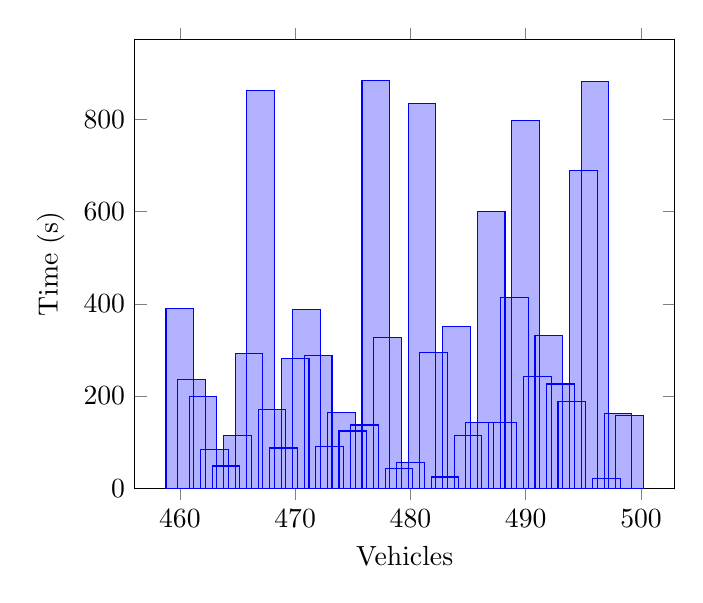
\begin{tikzpicture}
\begin{axis}[
legend style={anchor=west},
xlabel=Vehicles,
ylabel=Time (s),
ymin=0,
ybar,
]
\addplot coordinates {
(474, 165)
(489, 413)
(492, 331)
(467, 863)
(491, 243)
(480, 55)
(482, 294)
(481, 835)
(499, 158)
(497, 20)
(490, 798)
(469, 87)
(468, 170)
(472, 288)
(478, 327)
(462, 199)
(460, 389)
(483, 24)
(494, 188)
(495, 689)
(496, 883)
(493, 226)
(485, 115)
(470, 282)
(461, 236)
(473, 90)
(476, 137)
(488, 143)
(479, 42)
(465, 115)
(475, 124)
(466, 292)
(463, 84)
(484, 350)
(464, 48)
(487, 601)
(471, 387)
(486, 143)
(477, 885)
(498, 162)
};

\end{axis}
\end{tikzpicture}
\label{tik:time:100:53}
\caption{100 percent diving with GSC on route $53$}
\end{figure}
